%!TEX root = ../my_thesis.tex
\chapter{Caractérisation et identification des erreurs résiduelles} % (fold)

Texte intro

\vspace*{\fill}
\minitocTITI
\vspace*{\fill}
\newpage

\section{Existence des erreurs résiduelles}
Comme présenté dans le chapitre premier, l'apparition du plancher d'erreur dépend de la distribution des mots de codes 
possédant un faible poids \cite{distance_spectrum}. Plus encore, il a été montré que la zone du plancher d'erreur émanait 
de la présence \emph{d'erreurs résiduelles} \cite{takeshitaBCH}. 
La Figure \ref{fig:befe} présente l'évolution pour différentes valeurs de SNR du nombre de bits erronés par trame 
erronée pour quatre turbo codes du standard LTE et un du standard CCSDS. Dans tous les cas l'algorithme EML-MAP itérant 
jusque 8 fois est considéré. Il est visible que dans la zone de convergence, de nombreuses erreurs à l'issu du décodage
sont présentes. En revanche, dès lors que le décodeur fonctionne dans la zone du plancher d'erreurs, dans tous les cas
considérés, le nombre d'erreurs binaires par trame est inférieur à 10 en moyenne. De là, vient leur nom d'erreurs résiduelles.

\begin{figure}[!b]
	\centering
	\includegraphics[width=.8\textwidth]{main/ch3_fig/be/tikz/befe.pdf}
	\caption{Évolution du nombre moyens d'erreurs binaires par trame erronée pour différentes valeurs de SNR et différents
	turbo codes. Algorithme EML-MAP itérant jusque 8 fois. \label{fig:befe}}
\end{figure}

Une caractérisation de la distribution de ces erreurs 
résiduelles a été proposée dans \cite{residual_errors}. Cette dernière est basée sur les fonctions recenseuses de poids
(Weight Enumerator Functions ou WEF en anglais). En posant $P^{\langle ML\rangle}(m)$ la probabilité que $m$ bits soient 
erronés dans une trame, sachant que la trame est erronée après décodage à maximum de vraisemblance, il vient :
\begin{equation}
P^{\langle ML\rangle}(m) \simeq \frac{W^m~A_m^{\langle CP\rangle}(Z)\vert_{W=Z=e^{-RE_b/N_0}}}{\sum\limits_{w=1}^N W^w~A_w^{\langle CP\rangle}(Z) \vert_{W=Z=e^{-RE_b/N_0}}}
\label{eq:be1}
\end{equation}
où $A_w^{\langle CP\rangle}(Z)$ est le WEF conditionnel du turbo code considéré \cite{benedetto_unveiling}.

En considérant que les séquences d'information 
générant un mot de code de poids $w$ ont majoritairement le même poids, l'équation précédente peut alors être transformée en : 
\begin{equation}
P^{\langle ML\rangle}(m) \approx \frac{\displaystyle\sum\limits_{w, \frac{W_w}{A_w}=m} A_w\cdot \exp\left(-w R \frac{E_b}{N_0}\right)}
                  {\displaystyle\sum\limits_{w} A_w\cdot \exp\left(-w R \frac{E_b}{N_0}\right)}
\label{eq:be2}
\end{equation}
avec, comme déjà présenté dans le Chapitre Premier, $A_w$ le nombre de mots de codes de poids de Hamming $w$. La 
multiplicité des bits d'information $W_w$ est la somme des poids de Hamming des $A_w$ séquences binaires générant des
mots de codes de poids de Hamming $w$. Au prix d'un faible imprécision, cette forme de l'équation permet d'utiliser 
directement le spectre de distance d'un turbo code pour estimer le nombre de bits erronées dans le plancher d'erreur. Les
résultats obtenus alors avec cette équation différent alors légèrement de ceux obtenus avec l'Équation \ref{eq:be1}, puisque 
certaines valeurs sont masquées par l'opération de moyenne $\frac{W_w}{A_w}=m$.

Ainsi, le spectre de distance d'un turbo code permet de calculer la probabilité 
d'obtenir $m$ erreurs binaires dans un trame erroné en considérant un décodage ML pour un taux d'erreur suffisamment 
faible et un canal AWGN. De part la présence du terme en exponentielle, plus $w$ est distant de $d_{min}$, moins la 
multiplicité associée a un impact sur la distribution des erreurs résiduelles. Néanmoins, ceci peut être contre balancé 
par une multiplicité très importante (de l'ordre du millier).

Dans la section suivante, grâce à l'obtention des spectres de distances de différents turbo codes standardisés, une 
comparaison est menée quant à la distribution du nombre d'erreurs dans les trames erronées dans la zone du plancher d'erreurs.


\subsection{Distribution des erreurs résiduelles pour des turbo codes standardisés}
L'existence des erreurs résiduelles dans la zone du plancher d'erreur vient d'être établie. Une proposition d'obtention 
de la distribution de ces erreurs a été conjointement proposée. La Figure \ref{fig:be} présente la distribution des erreurs
résiduelles pour 5 turbo codes du standard LTE et un du standard CCSDS. Pour chacun de ces histogrammes, 500 trames erronées
après décodage via l'algorithme EMNL-MAP itérant 8 fois sont considérées. Pour tous ces codes, la très grande majorité des 
trames erronées contiennent moins de 10 erreurs binaires. Ceci est conforté par la Figure \ref{fig:befe}. Plus encore, 
hormis pour le turbo code du standard CCSDS, au moins 70\% des trames erronées ont strictement moins de 5 erreurs.

\begin{figure}[!ht]
	\centering
	\hspace*{-1cm}
	\includegraphics[width=1.07\textwidth]{main/ch3_fig/be/tikz/be.pdf}
	\caption{Distribution du nombre d'erreurs binaires pour différentes valeur de SNR et pour différents turbo codes des 
	standards LTE et CCSDS. 
	Décodage EML-MAP itérant 8 fois. \label{fig:be}}
\end{figure}

Sur cette Figure \ref{fig:be} sont aussi présentés les résultats théoriques obtenus pour la valeur de SNR la plus grande
grâce à l'équation \ref{eq:be1} et au spectre de distance calculé via la Double Impulse Method (cf. \ref{seq:spectre}).
Ces résultats sont aussi reportés pour plus de lisibilité dans le Tableau \ref{tab:theo}. Suivant le turbo code considéré,
des différences entre la valeur théorique et la valeur mesurée apparaissent. Néanmoins, la tendance calculée est conforme
aux mesures obtenues. Ainsi, la seule occurrence non prédite correspond à un BE de 1 pour le standard CCSDS, où $0.2\%$ 
était prédit alors que $11\%$ sont mesurés.

\begin{table}[]
\centering
\caption{Distribution théorique des erreurs dans le plancher d'erreur selon l'équation \ref{eq:be1} pour plusieurs turbo 
codes standardisés}
\label{tab:theo}
\resizebox{\textwidth}{!}{
\begin{tabular}{@{}lrrrrrrrrrrr@{}}
\toprule
                            & 1      & 2      & 3      & 4      & 5     & 6      & 7     & 8      & 9     & 10  & \textgreater10 \\ \cmidrule(r){1-1} \cmidrule(l){2-12}
LTE R=1/3, K=528 @ 2.4dB    & 33.9\% & 24.4\% & 29.3\% & 1.4\%  & 1\%   & 5.2\%  & 0.2\% & 0.02\% & 4.6\% & 0\% & 0\%            \\
LTE R=1/3, K=1024 @ 1.5dB   & 19.9\% & 32.7\% & 36.7\% & 6.2\%  & 3.6\% & 0.3\%  & 0.4\% & 0.2\%  & 0\%   & 0\% & 0\%            \\
LTE R=1/3, K=1504 @ 1.3dB   & 0\%    & 19.2\% & 68\%   & 8.3\%  & 2.2\% & 0.8\%  & 1.4\% & 0\%    & 0\%   & 0\% & 0\%            \\
LTE R=1/3, K=2048 @ 1.3dB   & 26\%   & 33.7\% & 30.2\% & 7.9\%  & 1.4\% & 0.3\%  & 0.4\% & 0.1\%  & 0\%   & 0\% & 0\%            \\
LTE R=1/3, K=6144 @ 0.8dB   & 0\%    & 76\%   & 7.2\%  & 14.2\% & 2.1\% & 0.3\%  & 0.1\% & 0\%    & 0\%   & 0\% & 0\%            \\
CCSDS R=1/3, K=1784 @ 1.3dB & 0.2\%  & 48.1\% & 27.9\% & 0.2\%  & 0.1\% & 22.3\% & 0.1\% & 0.1\%  & 0.6\% & 0\% & 0\%            \\ \bottomrule
\end{tabular}}
\end{table}

Afin de présenter la déviation entre la théorie développée dans la première section de ce Chapitre et les mesures 
effectuées, un calcul d'erreur quadratique moyenne (EQM, Équation \ref{eq:eqm}) est effectué pour chacun des turbo codes 
et est présenté dans le tableau \ref{tab:eqm}.

\begin{equation}
	EQM = \sqrt{\cfrac{1}{N}\sum\limits_{i=1}^N\bigl(T_i-M_i\bigr)^2}
	\label{eq:eqm}
\end{equation}

Les valeurs d'EQM sont alors comprises entre 3.8 et 9.5, impliquant que les valeurs théoriques et mesurées sont 
relativement proches. Les Équations \ref{eq:be1} et \ref{eq:be2} ne sont vraies que dans le cas d'un décodage 
ML, ne pouvant être effectué dans le contexte des turbo codes. Ce constat explique le léger écart relevé entre la 
théorie et les mesures.

Plus le ratio $\frac{W_d}{A_d}$ des premiers termes du spectre de distance du code est faible, plus le nombre moyen de 
bit erronés par trame erronée dans le plancher d'erreur sera faible lui aussi. D'autant plus, pour les turbo codes 
standardisés, les ratios $\frac{W_d}{A_d}$ sont faibles. Ceci implique alors un distribution des erreurs binaires dans 
le plancher d'erreur essentiellement sur les faibles nombres d'erreurs.
\begin{table}[b]
\centering
\caption{Erreur quadratique moyenne entre théorie et simulations Monte-Carlo}
\label{tab:eqm}
\resizebox{.4\textwidth}{!}{
\begin{tabular}{@{}lr@{}}
\toprule
                            & EQM \\
                      \cmidrule(r){1-1}      \cmidrule{2-2}
LTE R=1/3, K=528 @ 2.4dB    & 6.2 \\
LTE R=1/3, K=1024 @ 1.5dB   & 9.4 \\
LTE R=1/3, K=1504 @ 1.3dB   & 9.5 \\
LTE R=1/3, K=2048 @ 1.3dB   & 3.8 \\
LTE R=1/3, K=6144 @ 0.8dB   & 6.7 \\
CCSDS R=1/3, K=1784 @ 1.3dB & 6.9 \\
\bottomrule
\end{tabular}}
\end{table}

Finalement, lorsqu'un processus de décodage échoue dans le plancher d'erreur, la trame produite est très proche dans du 
mot de code transmis. Dans la section suivante, différents critères d'identification de ces erreurs résiduelles sont 
proposés et comparés.
\newpage
\section{Comparaison de critères d'identification}
Dans cette section, une comparaison de plusieurs métriques permettant l'identification des erreurs résiduelles est 
proposée. Ces métriques sont basés sur des quantités internes au turbo décodeur.\\
D'office, suite aux statistiques dressés dans le Chapitre précédent, des métriques utilisant des oscillations ne sont 
pas considérées. Ainsi, seules des métriques prenant en compte l'amplitude d'informations internes au turbo décodeurs 
sont considérées.

\subsection{Les différentes métriques considérées}
Dans le Chapitre précédent, il a été vu que le module de l'information \textit{a posteriori} peut être vu comme 
l'assurance du turbo décodeur sur sa décision quant à un certain bit du mot décodé. Ainsi, un première métrique pouvant 
être établie est la suivante :
\begin{equation}
	\Delta_1(k) = |L^a(k)|\text{~, avec k~}\in \llbracket0;~K \rrbracket 
\end{equation}
Aussi, il peut être considéré que de décorréler les informations du canal pour la métrique peut être intéressant. En effet, 
cela permet de n'exprimer que l'avis propre du décodeur. Cette métrique est alors basé uniquement sur les informations 
extrinsèques et a pour formule : 
\begin{equation}
	\Delta_2(k) = |L^e_{12}(k)+L^e_{21}(k)|
\end{equation}
D'autre part, il pourrait être intéressant de considérer une norme mathématique. L'évaluation de la norme 1 (distance de
Manhattan) est suffisante car le but de son emploi est d'ordonner les positions les moins probables. En effet, l'ordre est 
conservé quelque soit la norme p ($p \in \mathbb{N} $) employé. Les deux équations précédentes deviennent alors respectivement :
\begin{equation}
	\Delta_3(k) = |y^s(k)| + |L^e_{12}(k)| + |L^e_{21}(k)|
\end{equation}
et 
\begin{equation}
	\Delta_4(k) = |L^e_{12}(k)| + |L^e_{21}(k)|
\end{equation}

Pour toutes les métriques sus-cités, l'obtention des positions les moins fiables est réalisé en considérant celles pour 
lesquelles les métriques sont les plus faibles.

\subsubsection{Résultats d'identification}
Afin de comparer ces différentes métriques, des statistiques d'identification vont être dressées. Le protocole 
expérimental est le suivant. Après chaque itération du processus de turbo décodage, les $n$ positions les moins fiables
dans la trame sont extraites grâce à chacune des métriques. Si l'ensemble des erreurs est présente dans ces $n$ éléments,
alors l'identification est dite réussie. Les turbo codes considérés sont les mêmes que dans la section précédente, à 
savoir des turbo codes binaires du standard LTE et du standard CCSDS. Plusieurs valeurs de SNR sont présentés. Afin 
d'obtenir des données valides, 500 trames erronées après un décodage utilisant 8 itérations de l'algorithme EML-MAP sont
utilisées.

La Figure \ref{fig:id1024} présente les résultats pour le turbo code K=1024 et R=1/3. Cinq valeurs pour $n$ 
(correspondant à la profondeur de recherche) sont considérées, allant de 4 à 20. Tout d'abord, il est visible que 
les deux critères d'identification basés sur une norme ($\Delta_3$ et $\Delta_4$) présentent de moins bonnes performances
que les deux autres critères. Ceci peut être interprété en remarquant que les normes ne permettent pas d'identifier les
cas ou chacun des deux décodeurs possède un avis décidé (forte amplitude) mais différents (signes opposés). En revanche, 
les deux autres métriques identifient ces cas possibles. La même constatation est faite pour d'autre turbo codes. Ainsi, 
l'utilisation d'une norme (au sens mathématique) est écartée dans la suite, au profit des métriques $\Delta_1$ et $\Delta_2$.

Ces deux dernières possèdent des performances proches avec un avantage pour la métrique $\Delta_1$. Le pouvoir 
d'identification de ces deux métriques augmente lorsque la valeur de SNR augmente. Ceci est corrélé avec la diminution du 
nombre d'erreurs binaire par trame constatée dans la section précédente.

Toujours en considérant la Figure \ref{fig:id1024}, pour une valeur de SNR de 1.1 dB, entre 10 et 30\% des trames ont 
l'ensemble de leurs erreurs binaires identifiées, selon la profondeur de recherche employée. Cependant, ces taux ne 
permettent pas de proposer une correction intéressante. En effet, en supposant que ces 30\% de trames dont les erreurs sont 
identifiées sont effectivement corrigées par un mécanisme utilisant cette métrique, le taux d'erreur trame passerait alors 
de $2.3\times 10^{-4}$ à $1,6\times 10^{-4}$. Ainsi l'amélioration sur la courbe de performance ne serait que peu visible.

En considérant maintenant une valeur de SNR de 1.3 dB, le taux d'identification maximal atteint 65\% pour $n=20$ avec la 
métrique $\Delta_1$. Le taux d'erreur trame résultant de l'utilisation de cette métrique passerait alors de 
$1.5\times 10^{-5}$ à $5.2\times 10^{-6}$. Cette fois, des gains plus conséquents apparaîtraient. En comparaison, 
d'après les données de la Figure \ref{fig:be}, dans ce même cas expérimental, 71\% des trames ont 20 erreurs ou moins. 
Ainsi, par l'emploi de la métrique $\Delta_1$, 91\% des trames ayant moins de 20 erreurs ont toutes leurs erreurs 
identifiées. Ce taux passe à 83\% avec la métrique $\Delta_2$. Il peut donc être statué que le pouvoir d'identification 
de la métrique est très important. En effet, seules de rares trames à faibles erreurs binaires n'ont pas eu la position 
de leurs erreurs identifiées. Ainsi, les performances de la métrique sont d'autant plus importantes que le nombre de bits
erronés par trames erronées est faible. Cette assertion est vérifiée avec la valeur de SNR la plus élevée considérée.

En effet, pour une valeur de SNR de 1.5 dB, avec seulement une profondeur de recherche fixée à $10$, 87,6\% des 
trames erronées ont intégralité de leurs erreurs identifiées grâce à la métrique $\Delta_1$. Ce taux atteint 89,4\% avec 
la métrique $\Delta_2$. Pour cette valeur de SNR 93,8\% des trames possède 10 erreurs ou moins. Ainsi, les métriques 
permettent une identification quasiment parfaite de la position des erreurs résiduelles. Finalement, si chaque trame 
erronée dont la totalité des erreurs sont identifiées étaient corrigés, le taux trame résultant passerait de 
$3.6\times 10^{-6}$ à une valeur comprise entre $3.8\times 10^{-7}$ et $4.4\times 10^{-7}$ suivant la métrique employée.

\begin{figure}[!htb]
	\centering
	\includegraphics[width=.75\textwidth]{main/ch3_fig/id2/tikz/1024.pdf}
	\caption{Pourcentage d'identification pour le turbo code du standard LTE K=1024, R=1/3.
	Décodage EML-MAP itérant 8 fois. \label{fig:id1024}}
		\vspace*{-1cm}
\end{figure}
\newpage
La Figure \ref{fig:idLTE} présente les statistiques d'identification réussies pour trois autres turbo codes du standard 
LTE. Dans les trois cas considérés, les constations faites lors de l'analyse de la Figure \ref{fig:id1024} peuvent être 
réitérées. Ces histogrammes valident la pertinence des métriques $\Delta_1$ et $\Delta_2$ pour l'identification des bits 
erronés lors du processus itératif de décodage. Dans tous les cas, pour des valeurs correspondant à un fonctionnement des 
turbo décodeurs dans la zone du plancher d'erreur, au moins 90\% des trames erronées ont l'ensemble de leurs erreurs 
identifiées par la métrique $\Delta_1$ avec un profondeur de recherche de taille 6.

Dans la section suivante, les métriques proposées sont étendues et caractérisées dans le contexte de turbo codes double 
binaires.

\begin{figure}[!h]
	\centering
	\hspace*{-1cm}
	\includegraphics[width=1.05\textwidth]{main/ch3_fig/id2/tikz/lte.pdf}
	\caption{Pourcentage d'identification pour différents turbo codes du standard LTE K=528, K=2048 et K=6144 avec R=1/3.
	Décodage EML-MAP itérant 8 fois. \label{fig:idLTE}}
\end{figure}

\subsection{Extension des critères d'identification aux turbo codes double binaires}
Le décodage des turbo codes double binaires a été détaillé en section \ref{sec:dbl}. Pour rappel, lors de ce décodage par
l'algorithme EML-MAP, 4 valeurs extrinsèques sont échangés par symbole. En réalité, dans un but de simplification de 
l'architecture matérielle associée, ce ne sont que trois valeurs qui sont échangées puisqu'une normalisation vis-à-vis de 
la probabilité d'obtenir le symbole $\mathbf{0}$ est réalisée. 

La généralisation des métriques $\Delta_1$ et $\Delta_2$ au cas double binaire n'est pas trivial. Dans la suite, une 
extension permettant d'atteindre une identification au moins aussi que celle présentée précédemment est déroulée.
L'équation de la métrique $\Delta_1$ dans le cas binaire peut exprimée de la sorte : 
\begin{align*}
\Delta_1(k) &= |L^a(k)|\\
			&= |l^a_0(k)-l^a_1(k)|,
\end{align*}
où $l^a_b(k)$ représente la log-vraisemblance (LL) \textit{a posteriori} tel que le bit considéré prenne la valeur b. C'est à dire
$l^a_b(k) = log\left(P(\hat{b_k} = b)\right)$. Ceci peut alors être vu comme la distance entre les deux LLs de chaque symbole
binaire possible (0 et 1). L'extension au cas double binaire amènerai alors au calcul de 6 distances analogues puisque le
nombre de symboles est porté à 4 ($\mathbf{0}, \mathbf{1}, \mathbf{2}, \text{~et~} \mathbf{3}$). Ainsi, une combinaison 
de ces 6 distances serait nécessaire pour caractériser chaque symbole avec une valeur scalaire. Cette valeur devrait alors 
refléter la fiabilité du symbole considérée. Cependant, de tels calculs s'avèrent complexes à entreprendre. Il est alors 
proposé de ne considérer que les deux symboles les plus probables $S_{M_x}$ et $S_{M_y}$ qui maximisent $l^a_s$ :
\begin{align*}
S_{M_x}(k) &= \argmax\limits_{s\in\llbracket0;3\rrbracket}\left(l^a_s(k)\right) \\
S_{M_y}(k) &= \argmax\limits_{s\in\llbracket0;3\rrbracket\setminus{S_{M_x}(k)}}\left(l^a_s(k)\right)
\end{align*}
La métrique s'exprime alors :
\begin{equation}
	\Delta'_1(k) = l^a_{S_{M_x}}(k)-l^a_{S_{M_y}}(k)
\end{equation}

Avec un raisonnement similaire, la métrique analogue à $\Delta_2$ s'exprime alors : 
\begin{equation}
	\Delta'_2(k) = l^{e,\text{sum}}_{S_{M_x}}(k)-l^{e,\text{sum}}_{S_{M_y}}(k),
\end{equation}
avec
\begin{align*}
S_{M_x}(k) &= \argmax\limits_{s\in\llbracket0;3\rrbracket}\left(l^{e,\text{sum}}_s(k)\right) \\
S_{M_y}(k) &= \argmax\limits_{s\in\llbracket0;3\rrbracket\setminus{S_{M_x}(k)}}\left(l^{e,\text{sum}}_s(k)\right)
\end{align*}
et $l^{e,\text{sum}}_s(k) = \sum\limits_{p=1}^2l^e_{s,p}(k)$.

Dans les deux, cette métrique peut s'interpréter comme suit. Pour un position donnée $k$, si les LL des deux symboles les 
plus probables sont proches l'un de l'autre, la position $k$ est considérée comme moins fiable qu'une position pour
laquelle cette distance est plus grande.

\subsubsection{Résultats d'identification}
Le même protocole expérimental que celui décrit précédemment est exploité. Cependant des turbo codes du standard DVB-RCS
sont maintenant considérés. Le décodage utilise l'algorithme EML-MAP itérant 8 fois. Le facteur de remise à l'échelle 
vaut 0.5 pour les deux premières itérations et 0.85 pour les itérations suivantes. Les turbo codes considérés possèdent K=440
ou K=752 symboles d'informations. Les rendements considérés valent 1/3, 3/4 et 6/7. Ceci permet de couvrir un spectre 
relativement large des turbo codes double binaires à 8 états standardisés. 

La Figure \ref{fig:dvb752} présente les résultats d'identifications pour les cas K=752. Les résultats pour K=440 sont 
déportés en Annexe \ref{sec:ann3} pour une meilleure lisibilité.
\begin{figure}[!h]
	\centering
	\hspace*{-1cm}
	\includegraphics[width=1.05\textwidth]{main/ch3_fig/id2/dvb/tikz/752.pdf}
	\vspace*{-1em}
	\caption{Pourcentage d'identification pour différents turbo codes du standard DVB-RCS K=752, R=1/3, 3/4 et 6/7.
	Décodage EML-MAP itérant 8 fois. \label{fig:dvb752}}
\end{figure}
Cette Figure est sous-divisée en six sous-figures. La première ligne correspond aux cas R=1/3. Les mêmes propriétés 
identification que celles présentés dans le cas binaire apparaissent. Au fur et à mesure que la valeur du SNR croit, le 
taux identification augmente. La métrique basée sur l'information \textit{a posteriori} présente de meilleurs statistiques
d'identification que celle basée uniquement sur les informations extrinsèques. Cet écart diminue avec l'augmentation du SNR.
Finalement, avec une profondeur de recherche de 20 et pour une valeur de SNR de 2.2 dB, quelque soit la métrique considérée, 
plus de 95\% des trames erronées ont l'ensemble de leurs erreurs identifiées.

La deuxième ligne d'histogrammes présente quant à elle ces statistiques  pour un rendement de 3/4. Dans ce cas, la 
métrique basée uniquement sur les informations extrinsèques possède de moins bonnes performances que celle basée sur les 
informations \textit{a posteriori}. La même constatation est réalisée pour un rendement de 6/7. Ainsi, plus la rendement 
augmente, moins la métrique basée sur les informations extrinsèque est pertinente. Cette constatation est amplifiée pour 
de faibles valeurs de SNR. Cependant, dans tous les cas, la métrique basée sur les information \textit{a posteriori} 
possède de bonnes performances d'identification des erreurs résiduelles. En effet, un taux de plus de 90\% d'identification 
réussie est atteint dans la zone de convergence en considérant une profondeur de recherche de 20. 

En reprenant le calcul permettant d'obtenir l'information extrinsèque, il apparaît que cette dernière dépend essentiellement
de l'information de parité. Or, les turbo codes à fort rendement standardisé sont obtenues par le poinçonnage de l'information
de parité. Ceci esquisse alors une cause probable de l'avantage obtenu par la métrique $\Delta'_1$ sur la métrique $\Delta'_2$
lorsque le rendement augmente.

\subsection{Conclusions sur les métriques d'identification}
Faisant suite à la mise en exergue de l'existence d'erreurs résiduelles dans la région du plancher d'erreur des turbo codes,
différents métriques permettant l'identification de ces erreurs ont été proposées. Une comparaison des performances de ces 
différentes métriques a alors permis de sélectionner une métrique, nommée $\Delta_1$ (et $\Delta'_1$ pour son homologue 
adapté aux turbo codes double binaires). Celle-ci est basée sur la valeur absolue de l'information \textit{a posteriori}
et, permet d'obtenir des taux d'identification de 90\% dans la zone du plancher d'erreur pour une profondeur de recherche 
raisonnable, ce quelque soit le turbo code standardisé considéré. Ce taux de 90\% devrait permettre d'observer des gains 
de l'ordre d'une décade en considérant un algorithme tirant parti de cette métrique. La Section suivante a justement pour 
objet la proposition d'un tel algorithme.

\section{L'algorithme Flip'N'Check}
Cette section présente un algorithme permettant de tirer parti de la métrique sus-présentée. Tout d'abord, le 
principe de cet algorithme est détaillé. Ceci mène alors à la formalisation de ce dernier. Finalement, ces performances 
sont discutés dans le cadre de divers turbo codes standardisés.

\subsection{L'algorithme dans le cas des turbo codes binaire}

\subsubsection{Principe}
Dans un grand nombre de standards de communication numérique, le turbo code est concaténé en série avec un code CRC. En 
effet, à la différence d'un code LDPC, un turbo code ne peut détecter si la trame décidée est réellement un mot de code. 
L'algorithme  décrit ci-après va tirer conjointement parti des capacités de détection d'un code CRC et de la métrique 
d'identification précédente. 

Son principe est le suivant. Durant les $I_{\text{min}}$ premières itérations, le turbo décodeur itère sans que le code
CRC ne soit vérifié. Ceci permet d'éviter les faux positifs qui peuvent survenir lorsque la mot décodé est situé à une 
distance importante du mot de code transmis. Après l'itération $I_{\text{min}}$, si le code CRC est vérifié, le processus
s'arrête alors. Sinon, la fiabilité de chacun des bits systématiques est caractérisé en utilisant la métrique $\Delta_1$.
Les $q$ positions minimisant cette métrique sont alors extraits est stockés, dans $\Omega$. À partir de ces $q$ positions,
il est possible de générer $2^q-1$ mots candidats en inversant la décision prise par le décodeur. Pour chacun de ces 
candidats, le code CRC est testé. Si un de ces mot est un mot de code pour le CRC, alors le processus s'arrête. Sinon, 
l'itération suivante du processus de décodage est réalisé. Le processus est alors répété jusqu'à ce qu'un mot vérifie le 
CRC où jusqu'à ce que le nombre maximal d'itération soit atteint ($I_{TC}$). L'algorithme \ref{alg:fc_b} récapitule l'ensemble de 
ces opérations.

Dans cet algorithme, le paramètre $q$ est particulièrement important. Il détermine en effet le compromis entre performances
de décodage et complexité calculatoire. Ce paramètre définit la taille de l'espace de recherche des positions les moins
fiables. Une grande valeur de $q$ permet de d'identifier assurément plus d'erreurs, conformément à ce qu'il a été
présenté en Figures \ref{fig:idLTE} et \ref{fig:dvb752}. Néanmoins, lorsque $q$ est incrémenté de 1, le nombre de 
vérification de CRC est doublé.

Dans le suite, le choix est alors fait de fixer la valeur de $q$ à 10. De la sorte, selon les statistiques d'identification 
précédentes, une ordre de grandeur devrait être atteint sur les performances de décodages, ce sans trop impacter la complexité
calculatoire globale du décodage.

Dans la section suivante, une présentation des performances de décodage dans le cadre de turbo codes des standards LTE
et CCSDS est réalisée. Cet algorithme est nommé Flip'N'Check et abrégé en FNC dans la suite.

\begin{center}
\begin{minipage}{.86\textwidth}%
\begin{algorithm}[H]
\label{alg:fc_b}
	\DontPrintSemicolon
	\SetKwFunction{TD}{Itération de Turbo Décodage}
	\SetKwFunction{G}{GenerateTestPattern}
	\SetKwFunction{GC}{Génération du mot candidat}
	\SetKwFunction{L}{Extraction des positions les moins fiables}
	\SetKwFunction{R}{return}
	\SetKwFunction{CRC}{CRCheck}
	
	\For{i: 1 à  $I_{min}$}{
		\TD\;
	}
	\For{i: $I_{min}+1$ to  $I_{TC}$}{
		$\left(\mathbf{\hat{{d}}}, \mathbf{L}\right)$ = \TD\;
		\If{\CRC{$\mathbf{\hat{{d}}}$}==true}{
			\R{$\hat{{d}}$}\;
		}
		\Else{
			\For{k: 1 à K}{				
				$\Delta_k = |L_k|$\;		%
			}
			$\Omega =$ \L{$\Delta$, q}\;
			\For{j: 1 à $2^q-1$}{								
				$\mathbf{D} =$\GC{$\Omega, j, \mathbf{\hat{d}}$}\;
				\If{\CRC{$\mathbf{D}$}==true}{
					\R{$\mathbf{D}$}\;
				}
			}
		} %end else
	}
	\R{$\hat{{d}}$}\;
	\caption{L'algorithme Flip and Check pour les turbo codes binaires}
\end{algorithm}
\end{minipage}
\end{center}



\subsubsection{Performances de décodage}
Ces sections présente des résultats de simulations réalisées avec une représentation des données en virgule flottante.
Les tailles des trames considérés pour le standard LTE sont de 528, 1024, 2048 et 6144. Afin d'éviter les problèmes de
faux positifs liés à l'emploi du code CRC, la valeur de $I_\text{min}$ est fixée respectivement à 2, 3, 3 et 4. Le processus
de turbo décodage peut itérer jusque 8 fois. Enfin, la valeur de $q$ pour l'algorithme FNC est fixée à 8. La Figure 
\ref{fig:fnc_lte} présente une comparaison des performances entre décodage utilisant l'algorithme EML-MAP (courbes en 
traits pleins) à un décodage basé sur l'algorithme FNC (courbes en pointillés).

\begin{figure}[!htb]
	\centering
	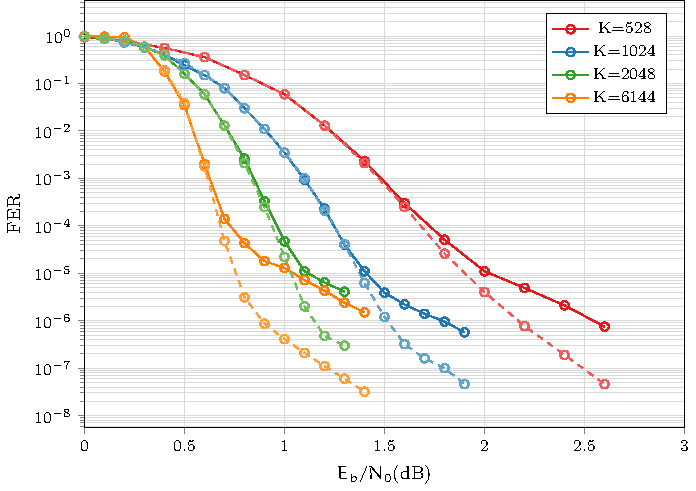
\includegraphics[width=\textwidth]{main/ch3_fig/fnc/lte/tikz/lte.pdf}
	\caption{Comparaison de performances de décodages entre EML-MAP et FNC. Standard LTE, K=528, 1024, 2048 et 6144.
	Décodeurs itérant 8 fois. \label{fig:fnc_lte}}
\end{figure}

Pour ces quatre cas considérés, l'amélioration du processus de turbo décodage obtenu par l'algorithme FNC représente un
gain en terme de FER au moins égal à un ordre de grandeur dans la zone du plancher d'erreur. Cela signifie qu'au moins 
$90\%$ des trames erronées sont corrigées par l'approche FNC. Le Tableau \ref{tab:fnccomp} compare le taux d'erreur trame 
attendu si l'ensemble des trames avec moins de 10 erreurs est corrigé et celui réellement obtenu avec l'algorithme FNC 
pour $q=10$. Ces données se basent sur celles de la Figure \ref{fig:be}. Il est toutefois à noter que pour les données de 
la Figure \ref{fig:be}, la redondance induite par le code CRC n'était pas considéré. En effet, le code CRC n'était alors 
pas utilisé dans le décodage. En revanche dans les courbes de la Figure \ref{fig:fnc_lte} il l'est soit en tant que 
critère d'arrêt, soit dans le processus FNC. Un décalage de la valeur du SNR par $10\times \log_{10}\left(\frac{K}{K-24}\right)$
est alors considéré pour présenter des données comparables.
\begin{table}[]
\centering
\caption{Comparaison entre les valeurs de taux d'erreur trames attendues avec une correction parfaite et celui réellement obtenu}
\label{tab:fnccomp}
\begin{tabular}{@{}lrrrr@{}}
\toprule
    & \begin{tabular}[c]{@{}l@{}}\textbf{K=528}  \\ @ 2.6 dB\end{tabular} & \begin{tabular}[c]{@{}l@{}}\textbf{K=1024} \\ @ 1.6 dB\end{tabular} & \begin{tabular}[c]{@{}l@{}}\textbf{K=2048} \\ @ 1.35 dB\end{tabular} & \begin{tabular}[c]{@{}l@{}}\textbf{K=6144} \\ @ 0.82 dB\end{tabular} \\ 
    \cmidrule(l){2-2}\cmidrule(l){3-3}\cmidrule(l){4-4}\cmidrule(l){5-5}
FER EML-MAP     & 7 e-7           & 2.3e-06         & 3e-6             & 4e-5             \\
BE < 10  		& 98\%            & 94\%            & 99\%             & 99\%             \\
FER attendu     & 1.4e-8          & 1.4e-7          & 3e-8             & 4e-7             \\
FER FNC         & 5e-8            &                 & 2e-7             & 2e-6             \\ \bottomrule
\end{tabular}
\end{table}
D'après ce tableau, il est visible que pour K=528 et K=1024, l'écart entre le taux d'erreur trame attendu et celui obtenu 
est relativement faible. En revanche, pour les deux autres longueur de trame, les performances sont un peu plus en retrait.
Ceci s'explique essentiellement par la capacité d'identification de la métrique. En effet, en comparant avec les statistiques d'identification fournies en Figure \ref{fig:idLTE}, les identifications réussies pour ces valeurs de SNR et longueurs de trame sont plus proches de 95\%
que des 99\%. Néanmoins, pour ces deux tailles de trames, les deux ordres de grandeurs de grandeurs de gains en terme de FER sont
approchés pour des valeurs de SNR plus élevés que celles considérés dans ce tableau \ref{tab:fnccomp}.

Finalement, à la vue de ces performances obtenues vis-à-vis de celles attendues, nous pouvons statuer sur l'absence de 
dégradations due à d'éventuels faux positifs émanant de la détection via le code CRC. Ceci provient conjointement de sa
distance minimale suffisamment importante (provenant directement de sa taille) et de l'adaptation de $I_{\text{min}}$ en 
fonction de la taille de la trame.

Les gains en terme de taux d'erreur binaire sont moins importants que ceux présentés pour le taux d'erreur trame. En effet,
de part son principe, l'algorithme FNC corrige les trames à faible nombre d'erreurs binaires. Ainsi, les trames erronées 
après processus FNC possèdent un nombre important d'erreurs binaires. Néanmoins, des gains d'environ un ordre de grandeur 
sont observés dans tous les cas considérés. 

La Figure \ref{}


Maintenant, un comparaison avec l'état de l'art sur des approches de 
basés sur un post-traitement est dressée.

\subsubsection{Comparaison avec l'état de l'art}

Commentaire sur l'identification\\
As tu mis une phrase sur le BER dans la section précédente ?

\subsection{L'algorithme dans le cas des turbo codes binaire}

\subsubsection{Les adaptations}

\subsubsection{Performances de décodage}




% Conclusion: Méthode relativement simple à mettre en oeuvre qui tire parti de l'auigmentation de la dmin du code grace a 
% la concat.

CONFIRMER VALEURS TABLEAU FNC